% \section{Рассмотрение случаев, когда алгоритм не сходится}

% На рисунке~\ref{fig:V_comp} изображены результаты работы известных алгоритмов по оценке многомерной медианы (Оджа, Тьюки и геометрическая), а также результаты 200 запусков предложенного алгоритма в следующих вариациях: с использованием относительного критерия (рис.~\ref{fig:V_rel}), с использованием относительного критерия и усреднением по последним 20 итерациям  (рис.~\ref{fig:V_rel_avg}), с экспоненциальным сглаживанием с $\alpha = 0,1$ и $c=5$ (рис.~\ref{fig:V_exp}), а также с экспоненциальным сглаживанием при тех же условиях и  усреднением по последним 20 итерациям (рис.~\ref{fig:V_exp_avg}). 

% На основе данных графиков можно заметить, что алгоритмы оценки медиан Тьюки, Оджа и геометрической сходятся примерно в одну точку, в то время как базовая версия (рис.~\ref{fig:V_rel}) предложенного алгоритма демонстрирует значительный разброс оценок, формируя хаотичное облако точек. Если же добавить усреднение по последним итерациям  (рис.~\ref{fig:V_rel_avg}), то разброс уже не такой выраженный и полученные оценки образуют более однородное и компактное облако. 


% Применение экспоненциального сглаживания приводит к еще большему уменьшению разброса (рис.~\ref{fig:V_exp}), размеры облака становятся заметно меньше. Если же еще добавить усреднение (рис.~\ref{fig:V_exp_avg}), то результаты хоть и незначительно, но все же еще улучшатся и разброс значений по оси y не будет превышать $0,1$, что является существенным улучшением по сравнению с исходной ситуацией. 


% \begin{figure}[h]
%   \centering
%   \begin{subfigure}[b]{0.4\textwidth}
%     \centering
%     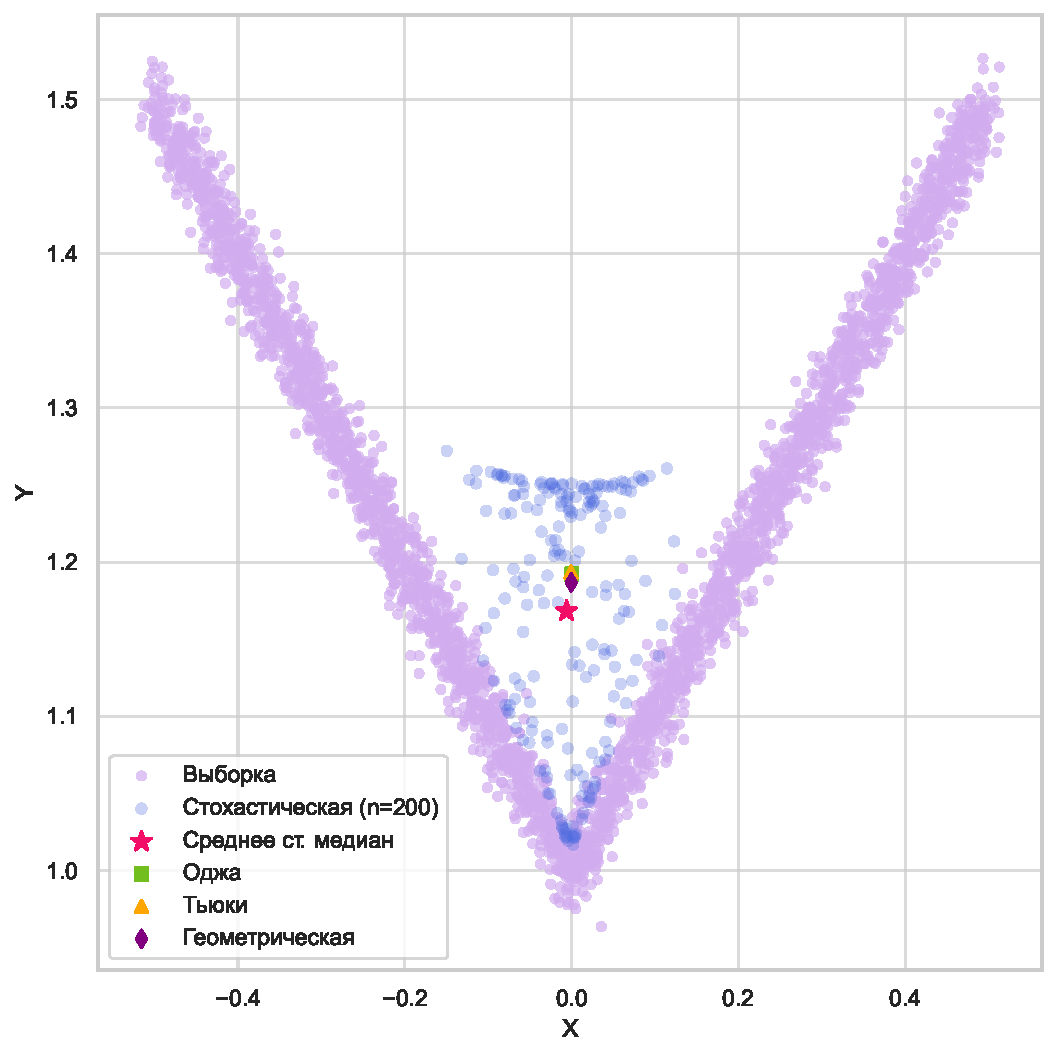
\includegraphics[width=\textwidth]{sample_V_base.pdf}
%     \captionsetup{labelformat=empty}
%      \caption{(a) Base}
%      \label{fig:V_rel}
%   \end{subfigure}
%   \begin{subfigure}[b]{0.4\textwidth}
%     \centering
%     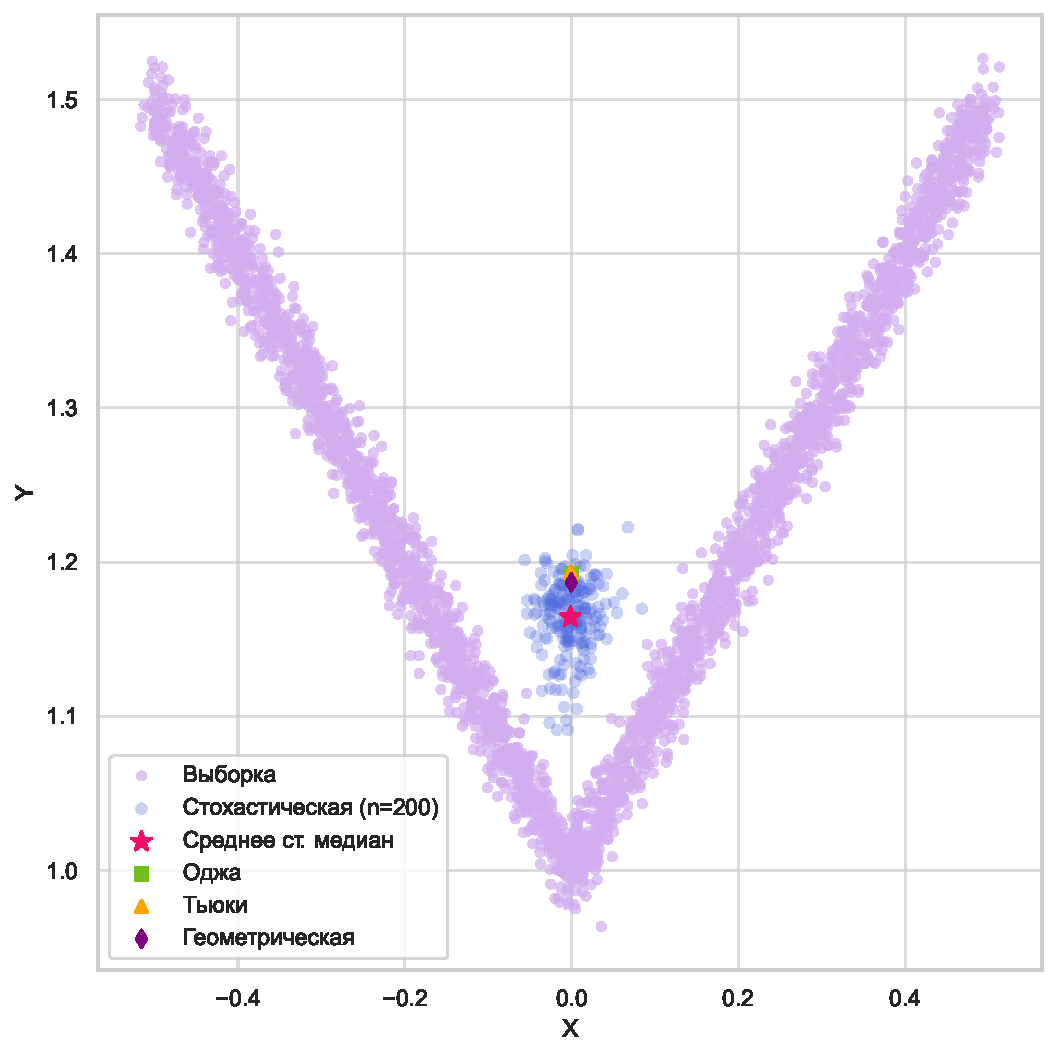
\includegraphics[width=\textwidth]{sample_V_base_avg.pdf}
%     \captionsetup{labelformat=empty}
%     \caption{(d) Base + Avg}
%    \label{fig:V_rel_avg}
%   \end{subfigure}
%   \begin{subfigure}[b]{0.4\textwidth}
%     \centering
%     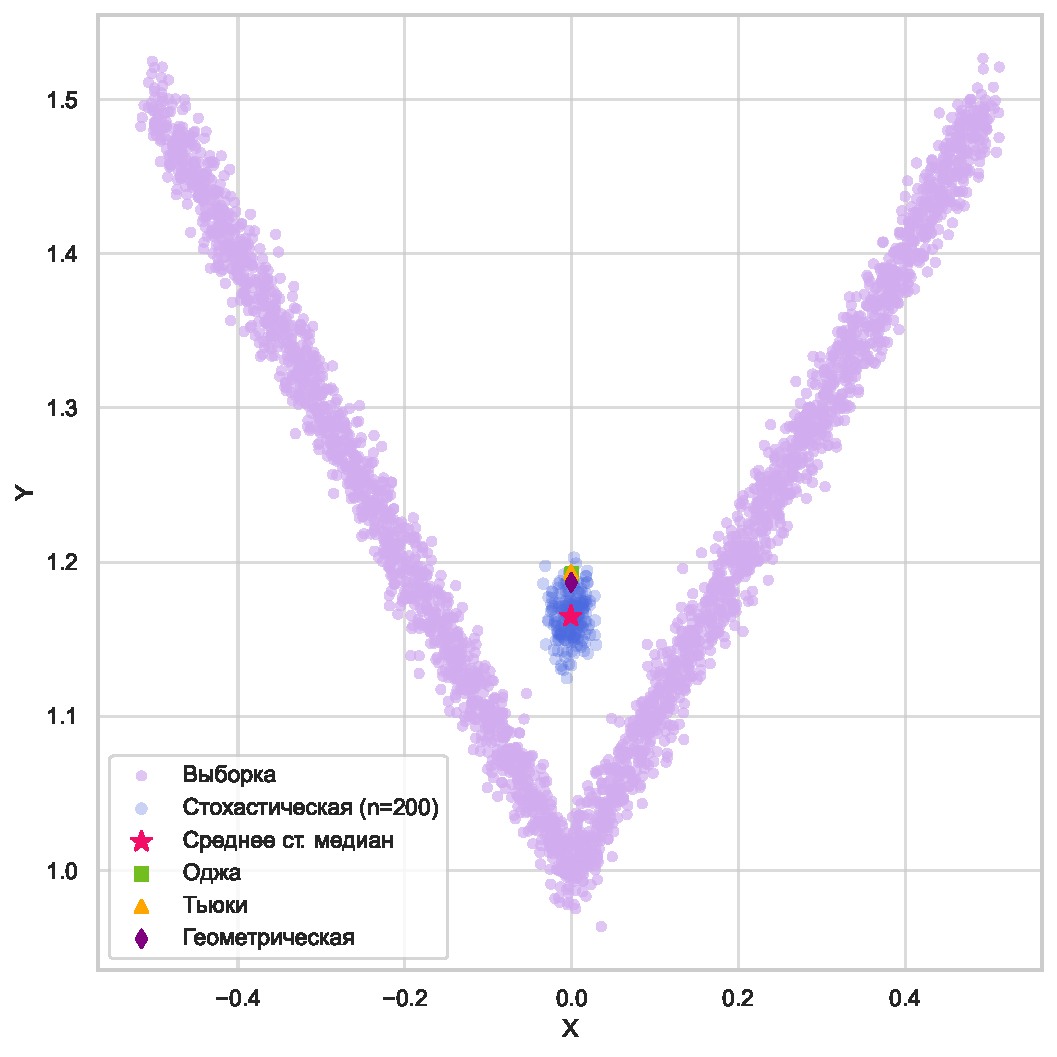
\includegraphics[width=\textwidth]{sample_V_exp.pdf}
%     \captionsetup{labelformat=empty}
%      \caption{Exp}
%      \label{fig:V_rel_exp}
%   \end{subfigure}
%   \centering
%   \begin{subfigure}[b]{0.4\textwidth}
%     \centering
%     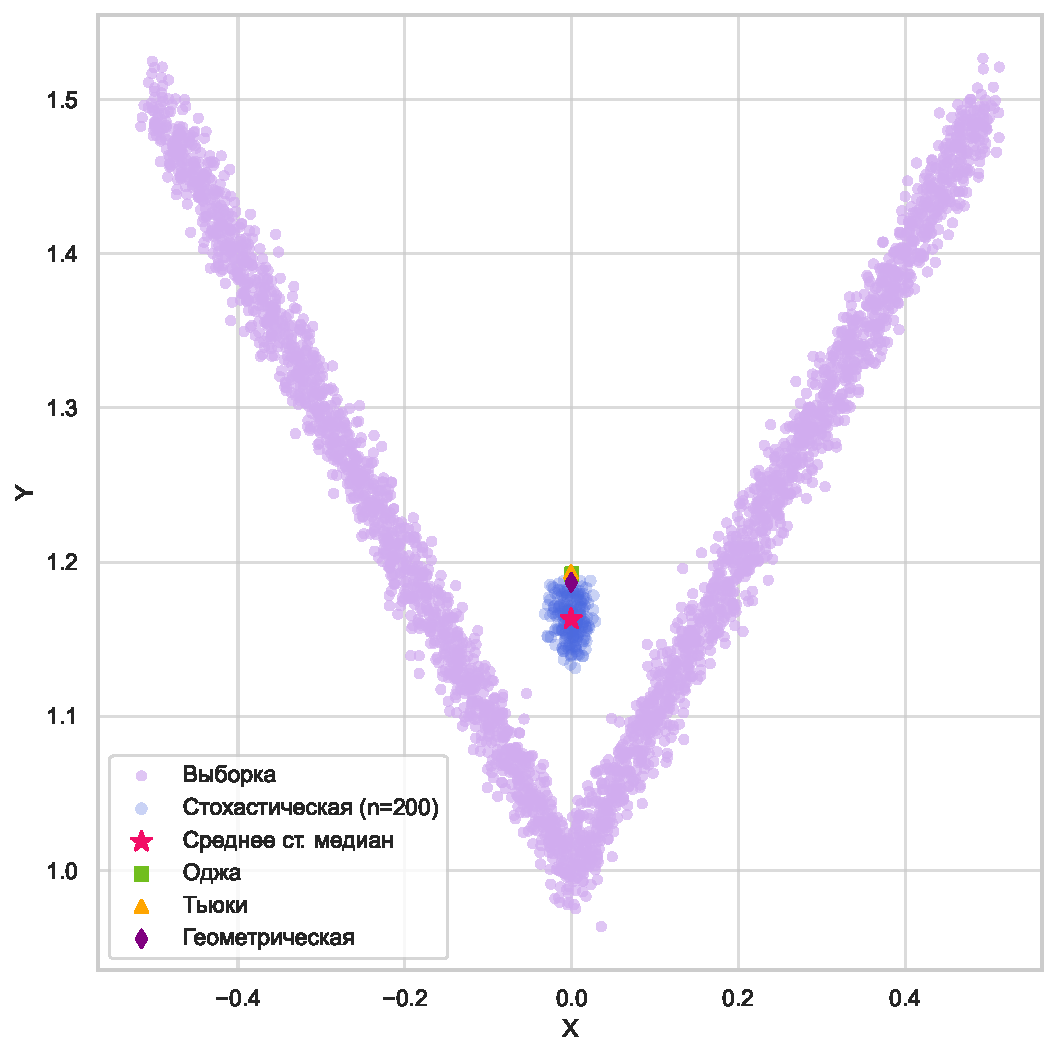
\includegraphics[width=\textwidth]{sample_V_exp_avg.pdf}
%     \captionsetup{labelformat=empty}
%      \caption{Exp + Avg}
%      \label{fig:V_rel_exp_avg}
%   \end{subfigure}
%   \begin{subfigure}[b]{0.4\textwidth}
%     \centering
%     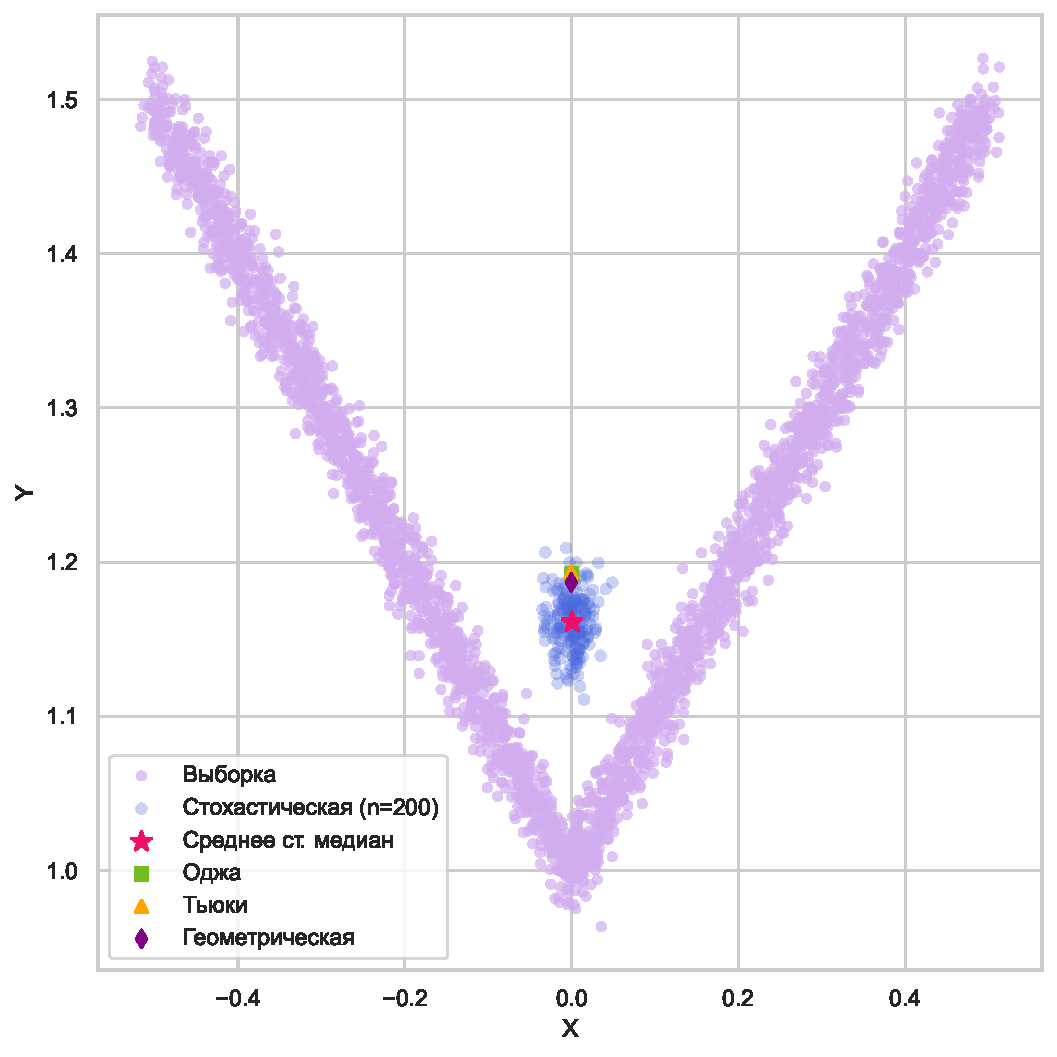
\includegraphics[width=\textwidth]{sample_V_ada.pdf}
%     \captionsetup{labelformat=empty}
%     \caption{(c) Ada}
%     \label{fig:V_rel_ada}
%   \end{subfigure}
%   \begin{subfigure}[b]{0.4\textwidth}
%     \centering
%     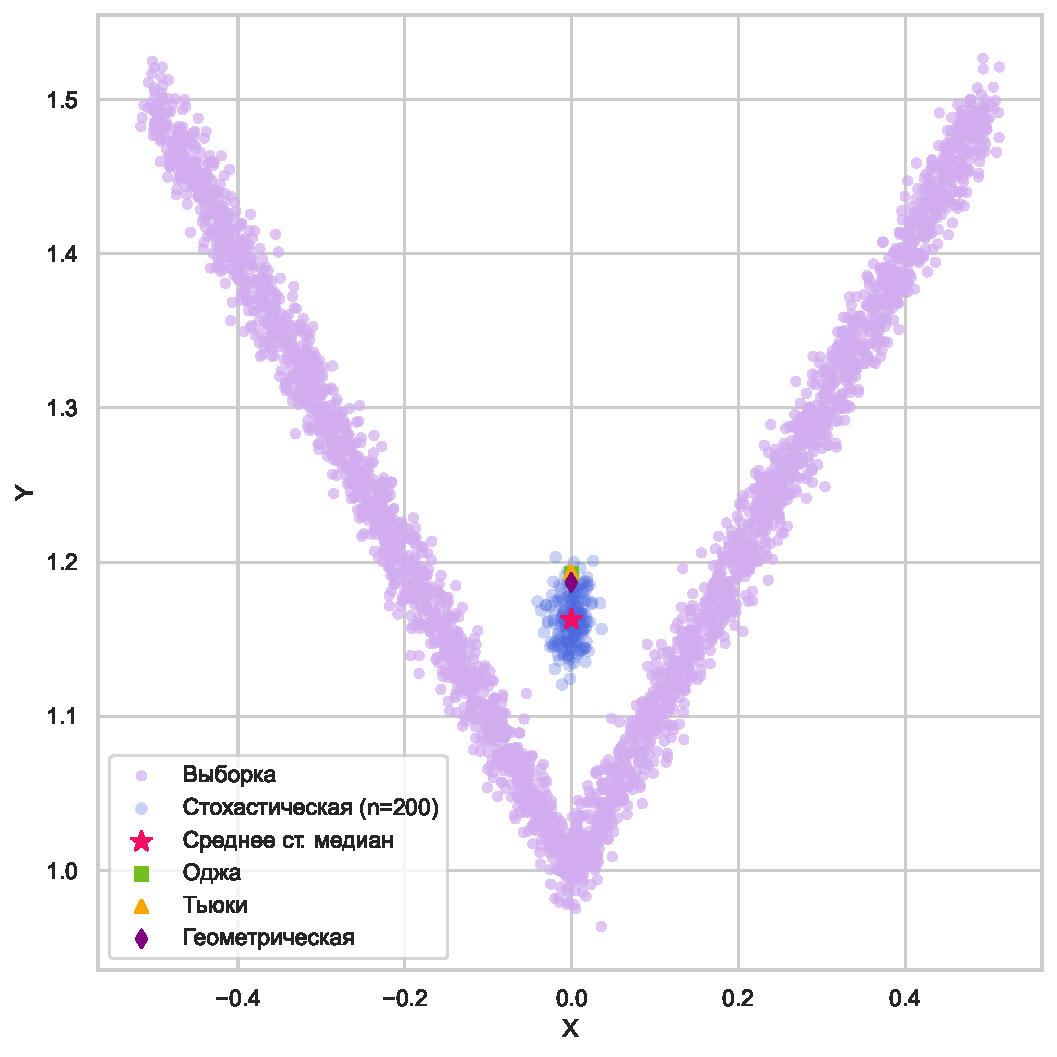
\includegraphics[width=\textwidth]{sample_V_ada_avg.pdf}
%     \captionsetup{labelformat=empty}
%      \caption{(f) Ada + Avg}
%      \label{fig:V_rel_ada_avg}
%   \end{subfigure}
%   \caption{Результат работы различных модификаций алгоритма на выборке, образующей букву V.}
%  \label{fig:V_comp}
% \end{figure}

% Рассмотрим также поведение алгоритма на выборке, образующей букву C. На этот раз сравним результаты, полученные при использовании относительного критерия останова, с результатами, полученными при использовании экспоненциального сглаживания и усреднения с параметрами, аналогичными использованным в предыдущем примере. 

% На рисунке~\ref{fig:C_comp} представлены результаты, демонстрирующие оценки многомерной медианы, полученные различными алгоритмами. Видно, что медианы Тьюки, Оджа, геометрическая, а также среднее значение, полученное на основе результатов работы стохастического алгоритма, сходятся к близким значениям. При этом сходимости для самой стохастической медианы в случае использования только относительного критерия не наблюдается (рис.~\ref{fig:C_rel}), так как полученные в результате работы алгоритма значения образуют облако с заметным разбросом точек внутри него. Если же рассматривать модификацию с экспоненциальным сглаживанием и усреднением (рис.~\ref{fig:C_exp_avg}), то облако становится существенно меньше, что позволяет сделать вывод о приблизительной сходимости алгоритма в данном случае.

% \begin{figure}[!hhh]
%   \centering
%   \begin{subfigure}[b]{0.45\textwidth}
%     \centering
%     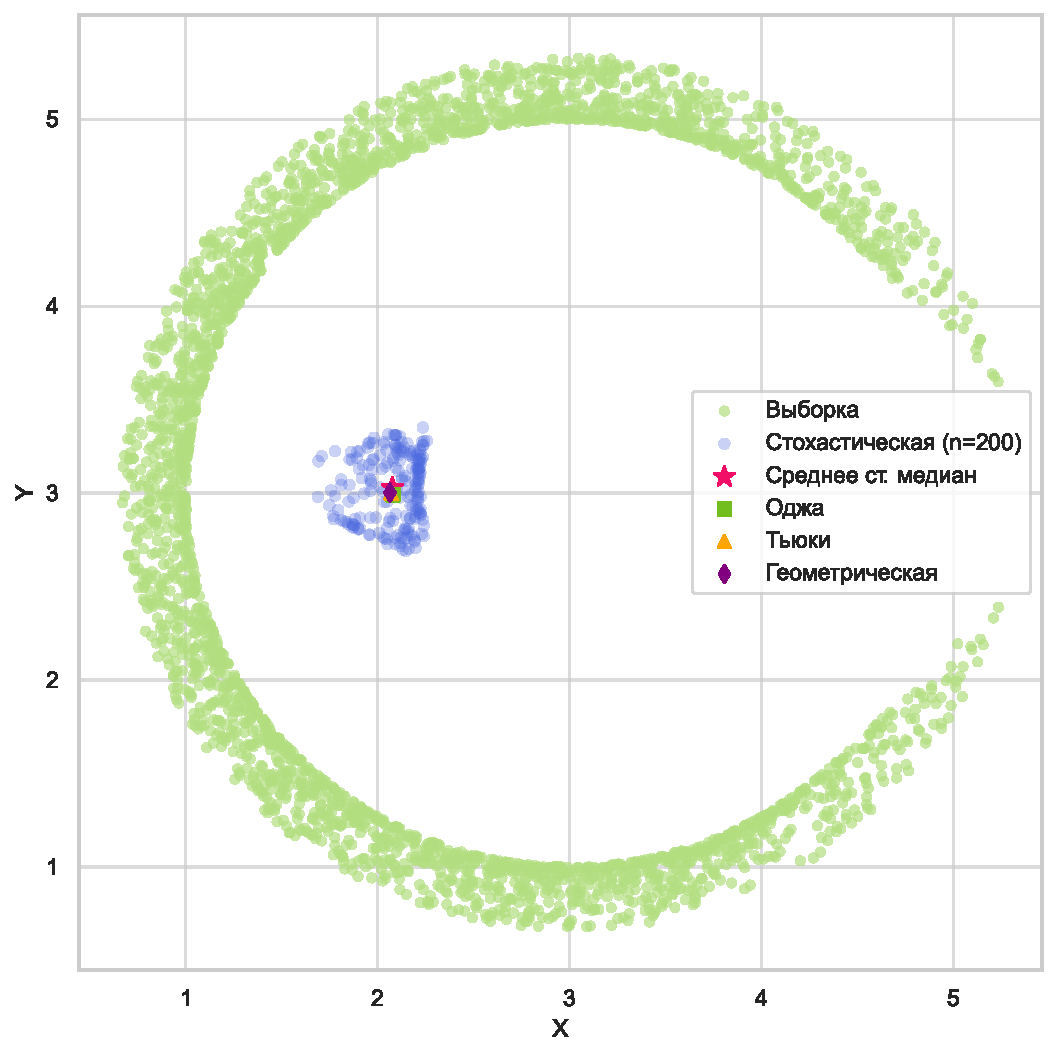
\includegraphics[width=\textwidth]{sample_C_base_new.pdf}
%     \captionsetup{labelformat=empty}
%      \caption{(a) Base}
%      \label{fig:C_rel}
%   \end{subfigure}
%    \hfill
%   \begin{subfigure}[b]{0.45\textwidth}
%     \centering
%     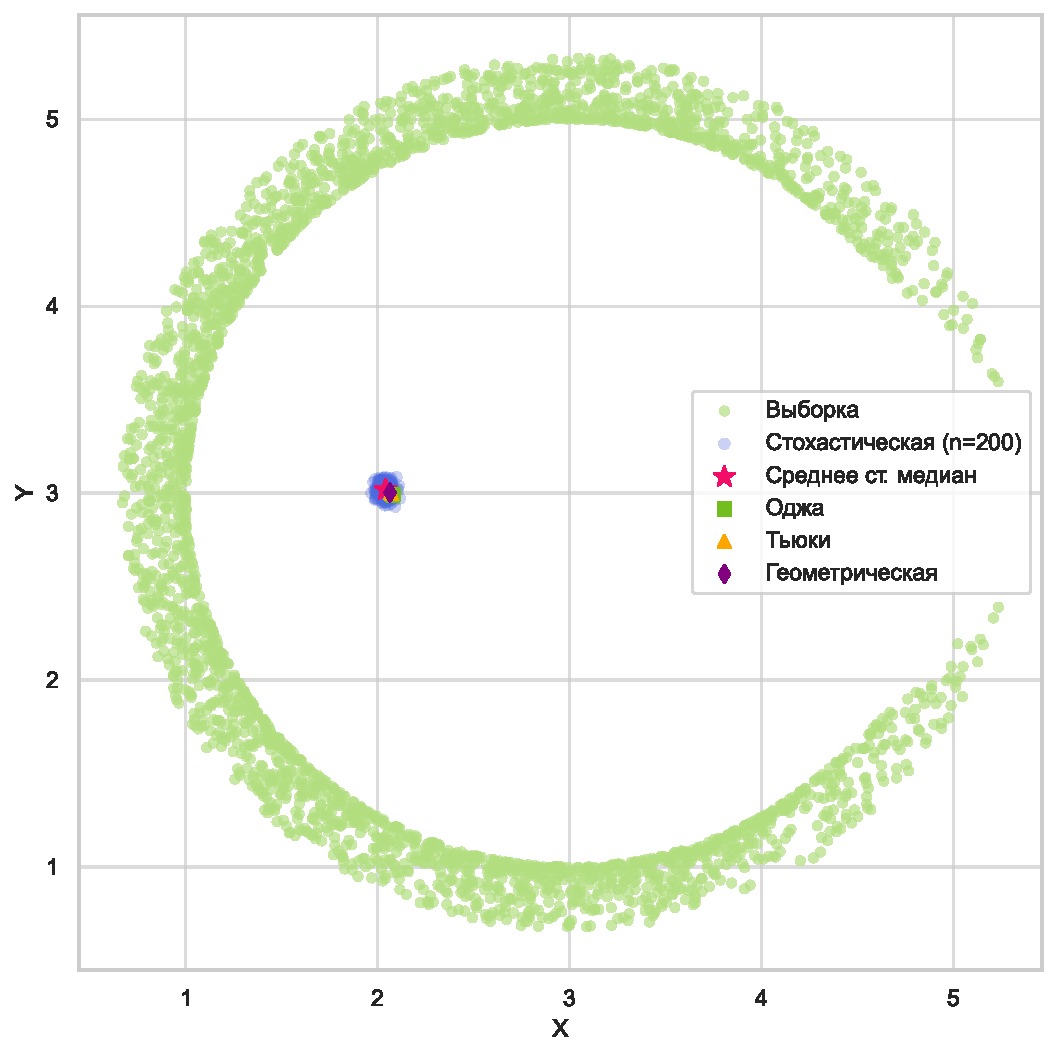
\includegraphics[width=\textwidth]{sample_C_exp_avg.pdf}
%     \captionsetup{labelformat=empty}
%     \caption{(b) Exp + Avg}
%     \label{fig:C_exp_avg}
%   \end{subfigure}

%   \caption{Результат работы различных модификаций алгоритма  на выборке, образующей букву C. }
%  \label{fig:C_comp}
% \end{figure}

% \newpage

% Рассмотрим двумерную выборку из $9$ точек, которые задают вложенные равносторонние треугольники на плоскости:
% \[
% (3; 2), \ (4; 3),\ (5; 4),\ (11; 2),\ (10; 3),\ (9; 4), \ (7; 2+ 4 \cdot \sqrt{3}),\ (7; 3+ 3 \cdot \sqrt{3}), \ (7; 4+ 2 \cdot \sqrt{3}).
% \]
% Центр тяжести в данном случае находится в точке $\left(7 \;\;   \frac{4\cdot\sqrt{3}}{6} + 4\right)^{\mathrm{T}}.$

% \vspace{1ex}

% % На рисунке \ref{fig:point_9} показаны результаты работы предложенного алгоритма и известных алгоритмов оценки параметра положения.   Алгоритмы, вычисляющие медиану Тьюки и геометрическую, дают наиболее близкие к ожидаемому результаты. Среднее также дает приемлемый результат. Медиана Оджа в данном случае далека от центра тяжести. 

% Предложенный стохастический алгоритм на данной выборке не сходится.  В этом можно убедиться, посмотрев на траекторию, которая является хаотичной (Рисунок \ref{fig:point_9_traj}). Алгоритм <<скачет>> от вершины к вершине внутреннего самого маленького треугольника и не может сойтись к центру тяжести.  

% \begin{figure}[!hhh]
%    \centering
%     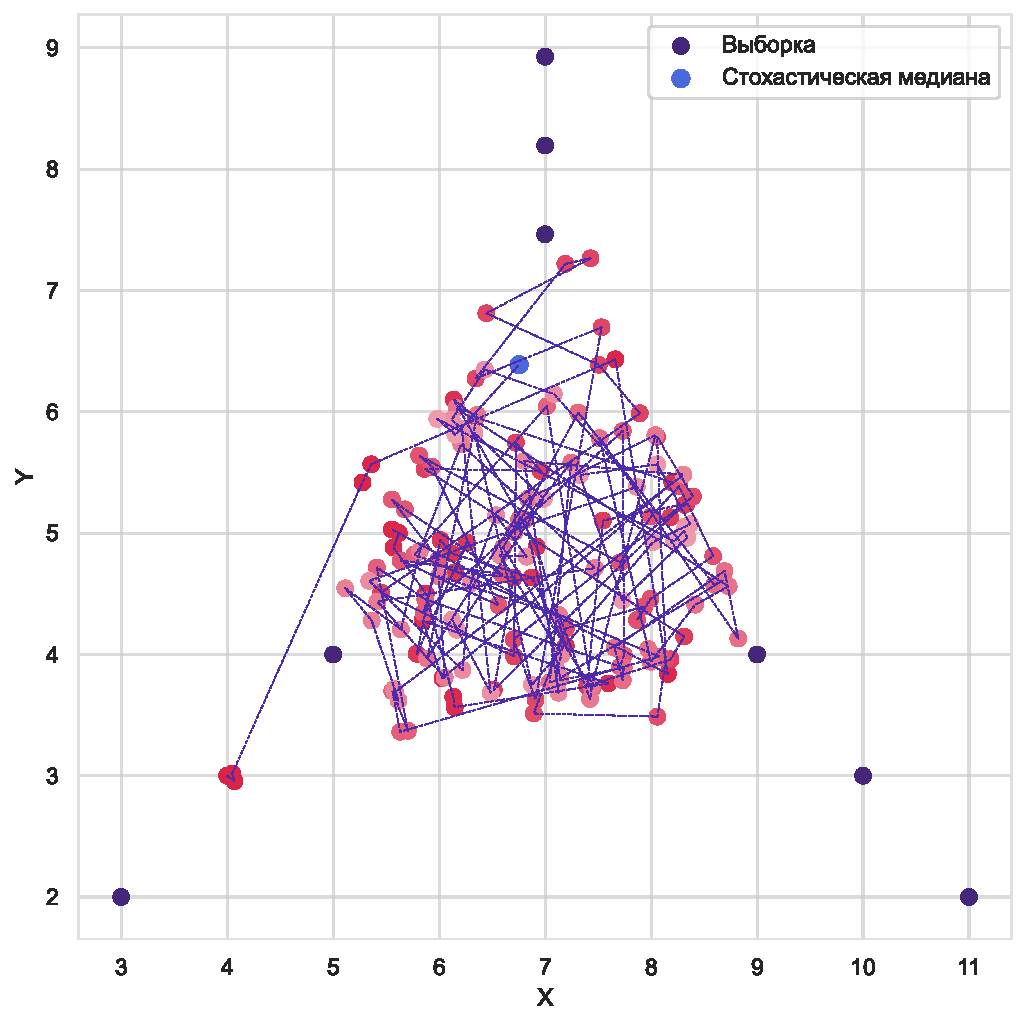
\includegraphics[width=0.6\textwidth]{sample_9point_4.pdf}
%   \caption{Траектория стохастического алгоритма для выборки из 9 точек.}
%   \label{fig:point_9_traj}
% \end{figure}

% % Посмотрим также на гистограмму ошибок на Рисунке \ref{fig:point_9_hist}, где ошибка определяется как разность полученного результата и мат. ожидания. На основе гистограммы можно сказать, что в большинстве случаев алгоритм скачет именно между тремя внутренними точками (так как в данном случае норма ошибки равна $\approx 1$--$1,5$).

% % \begin{figure}[!hhh]
% %    \centering
% %     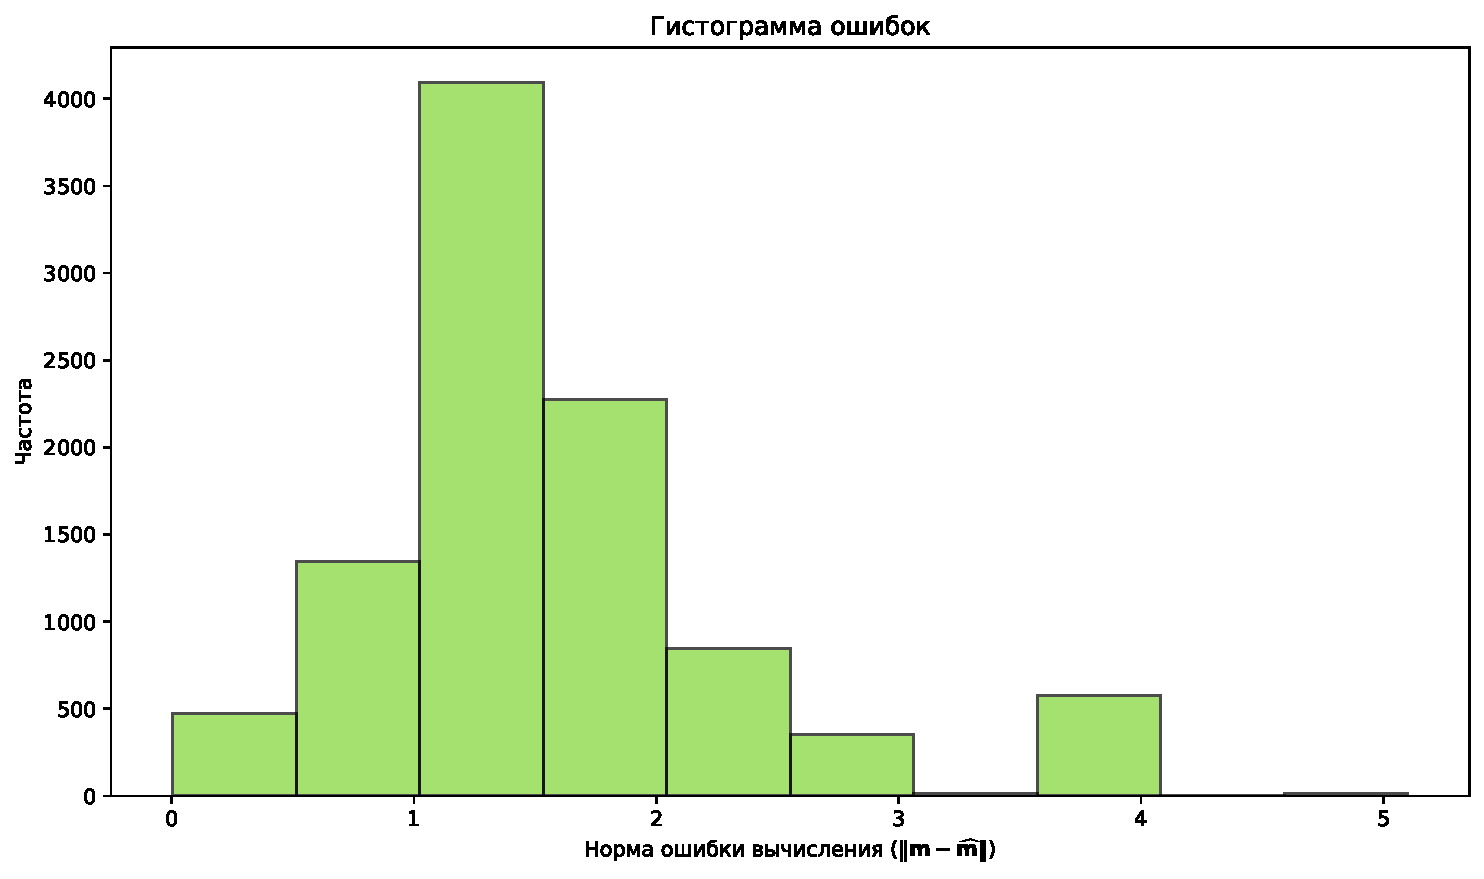
\includegraphics[width=14cm]{hist_9point.pdf}
% %   \caption{Алгоритм запускается 10000 раз на выборке из 9 точек. На основе полученных результатов строится гистограмма ошибок.}
% %   \label{fig:point_9_hist}
% % \end{figure}


% Анализ рисунка~\ref{fig:9point_comp} показывает, что на выборке, состоящей из вершин вложенных равносторонних треугольников, базовая версия алгоритма (рис.~\ref{fig:9point_rel}) не обеспечивает сходимость. Оценки <<скачут>> внутри треугольника, образованного самыми внутренними вершинами.

% Применение экспоненциального сглаживания значительно улучшает ситуацию (рис.~\ref{fig:9point_exp_avg}): выборка оценок образует компактное облако точек. При этом отклонение по каждой из осей от его центра (среднего значения полученных оценок) не превышает единицы, что свидетельствует о существенном повышении устойчивости алгоритма.

% \begin{figure}[!hhh]
%   \centering
%   \begin{subfigure}[b]{0.45\textwidth}
%     \centering
%     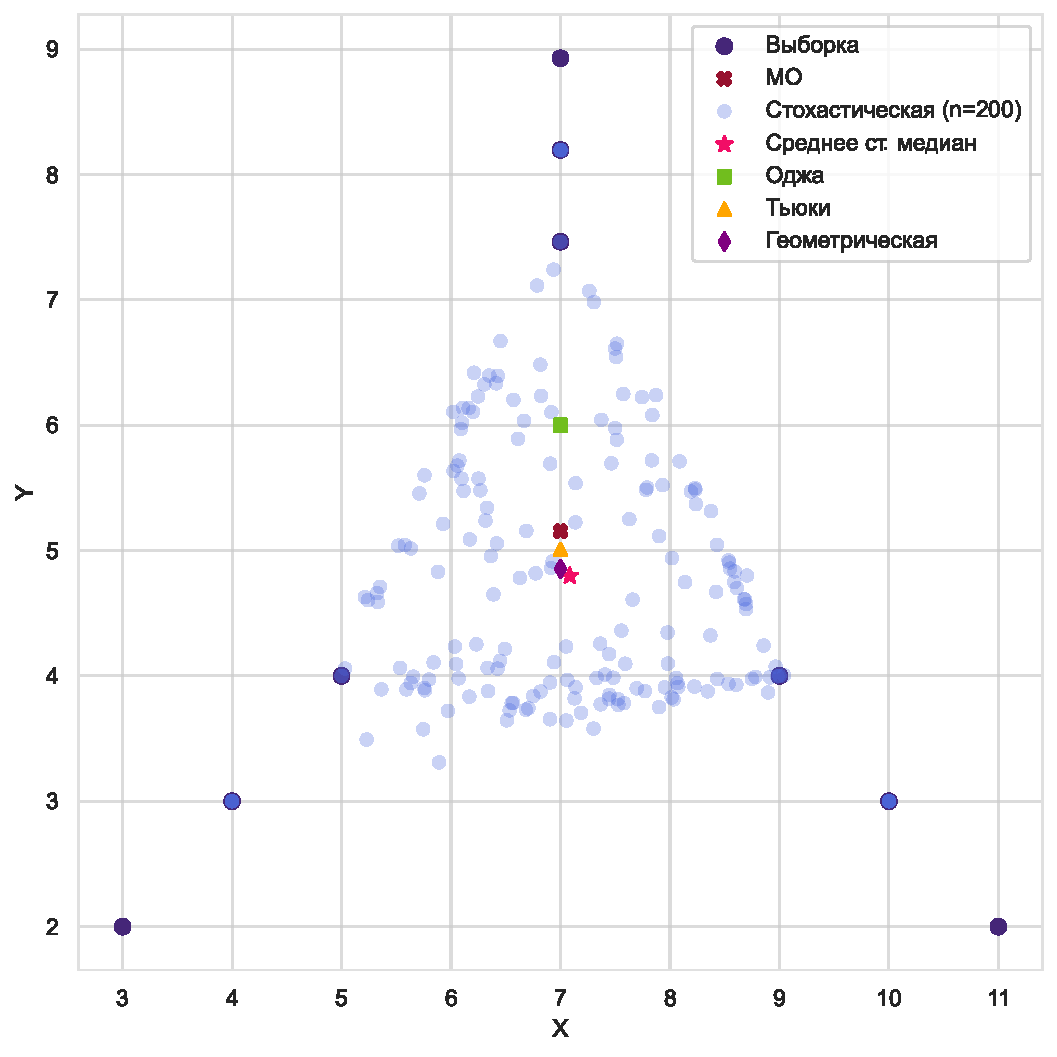
\includegraphics[width=\textwidth]{sample_9point_rel_crit_new.pdf}
%     \captionsetup{labelformat=empty}
%      \caption{(a) Base}
%      \label{fig:9point_rel}
%   \end{subfigure}
%    \hfill
%   \begin{subfigure}[b]{0.45\textwidth}
%     \centering
%     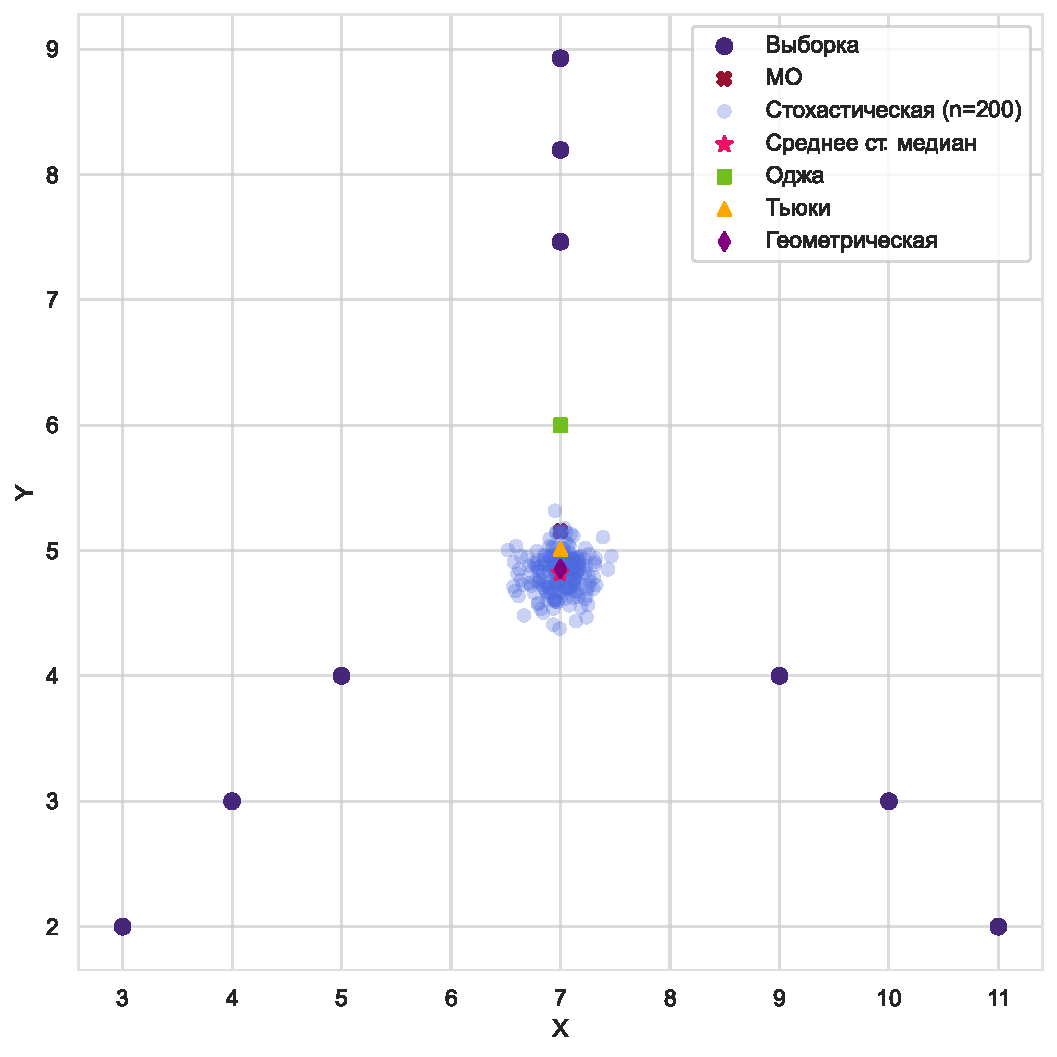
\includegraphics[width=\textwidth]{sample_9point_rel_crit_ada.pdf}
%     \captionsetup{labelformat=empty}
%     \caption{(b) Ada + Avg}
%     \label{fig:9point_exp_ada}
%   \end{subfigure}

%   \caption{Результат работы модификаций алгоритма на выборке из 9 точек --- вершин вложенных равносторонних треугольников.}
%  \label{fig:9point_comp}
% \end{figure}


\section{Рассмотрение случаев отсутствия сходимости алгоритма}

В предыдущих разделах было показано, что предложенные модификации позволяют уменьшить разброс оценок и повысить устойчивость алгоритма на выборках из стандартных распределений. Однако представляет интерес исследование случаев, в которых стохастический алгоритм испытывает трудности со сходимостью.

Далее рассматриваются несколько примеров выборок со сложной формой, для которых базовая версия алгоритма демонстрирует неустойчивое поведение. Основное внимание уделяется сравнению различных модификаций алгоритма и анализу того, насколько они позволяют уменьшить разброс оценок.

\subsection{Выборка, образующая букву V}

На Рисунке~\ref{fig:V_comp} представлены результаты работы различных модификаций алгоритма на выборке, образующей букву V. Для каждой модификации проводилось $200$ независимых запусков алгоритма.

Рассматриваются следующие варианты алгоритма:
\begin{itemize}
    \item базовая версия алгоритма с относительным критерием останова (Base);
    
    \item базовая версия с усреднением последних итераций (Base + Avg);
    
    \item алгоритм с экспоненциальным сглаживанием (Exp);
    
    \item алгоритм с экспоненциальным сглаживанием и усреднением (Exp + Avg);
    
    \item алгоритм с адаптивным выбором шага AdaGrad (AdaGrad);
    
    \item алгоритм AdaGrad с усреднением (AdaGrad + Avg).
\end{itemize}

Во всех случаях использовались многократное выполнение критерия останова и ограничение на минимальное число итераций, которое должен отработать алгоритм.

\begin{figure}[!htbp]
  \centering
  \begin{subfigure}[b]{0.32\textwidth}
    \centering
    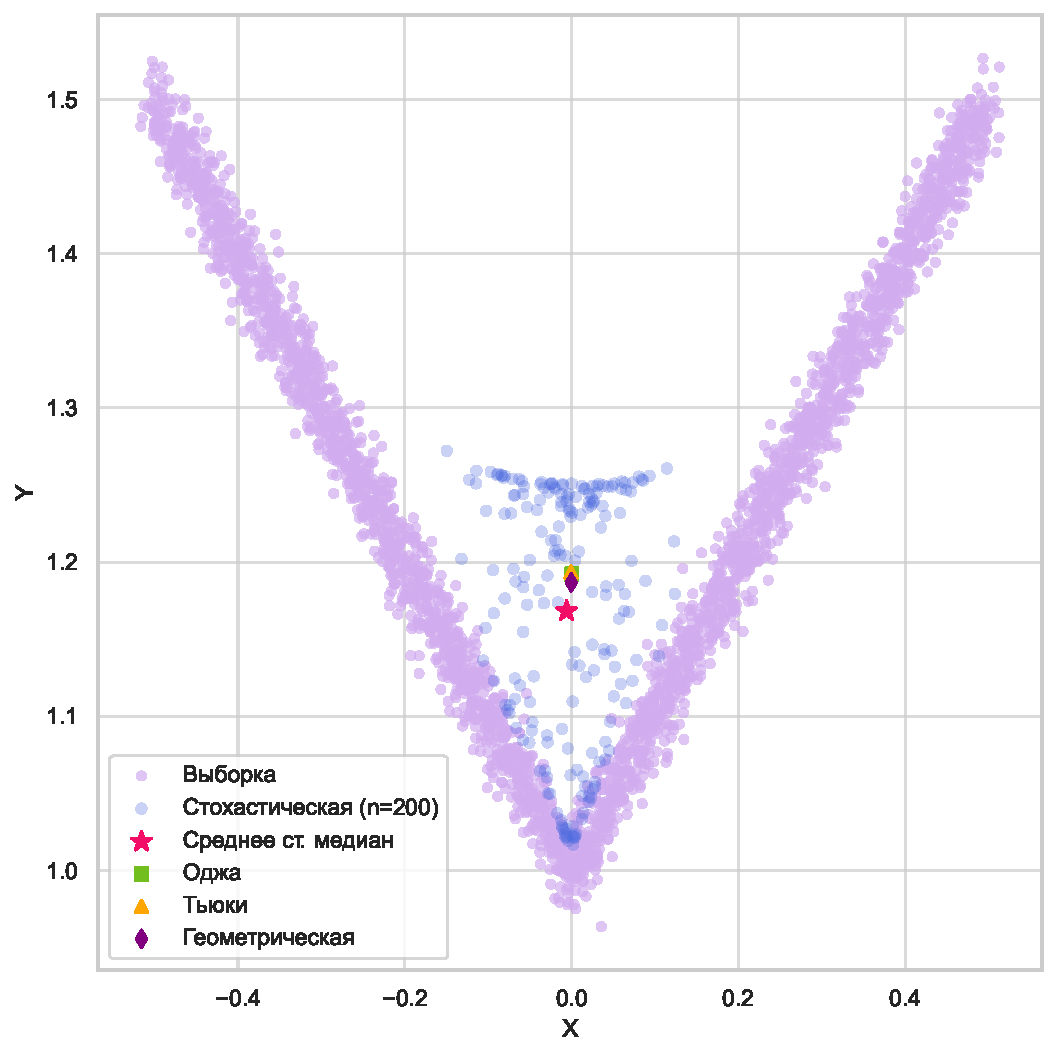
\includegraphics[width=\textwidth]{sample_V_base.pdf}
    \captionsetup{labelformat=empty}
     \caption{(а) Base}
     \label{fig:V_rel}
  \end{subfigure}
  \hfill
  \begin{subfigure}[b]{0.32\textwidth}
    \centering
    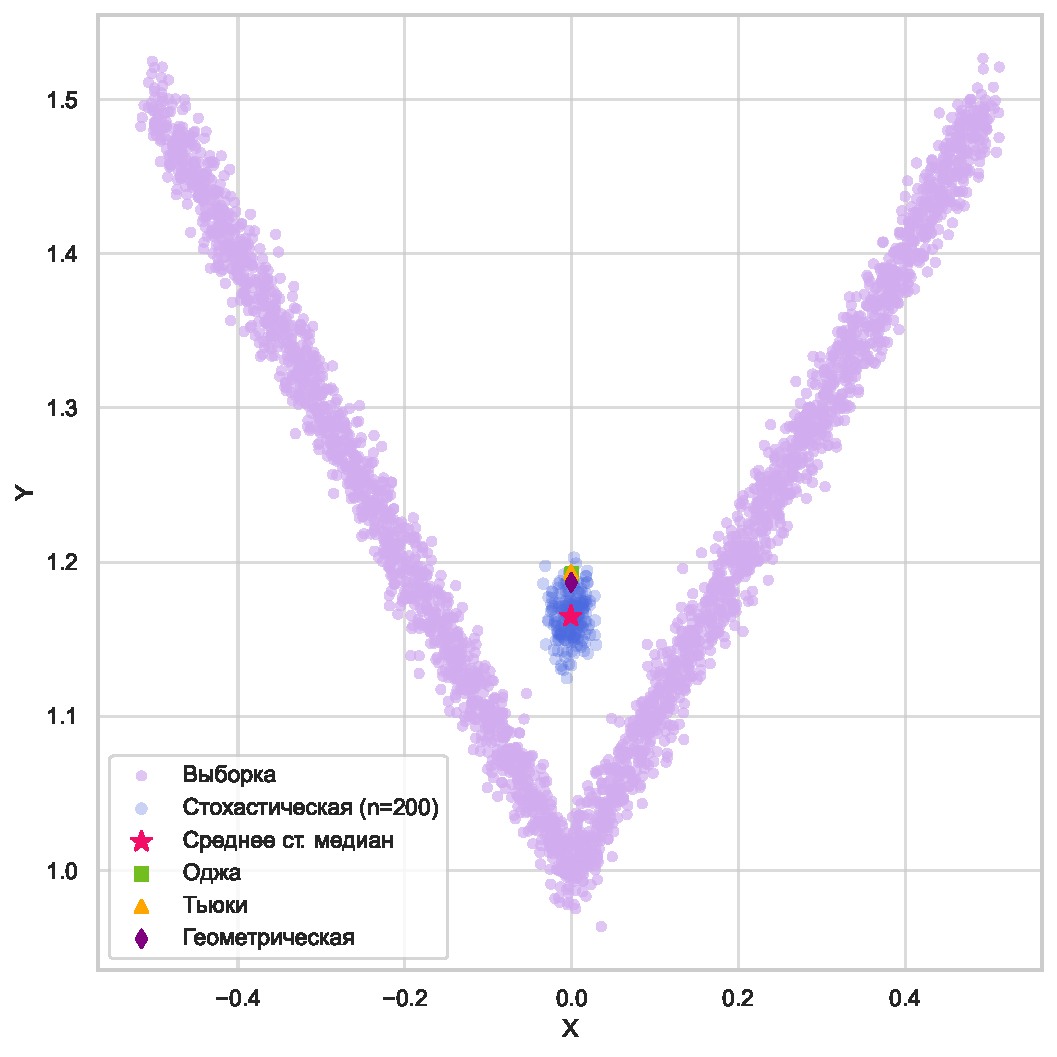
\includegraphics[width=\textwidth]{sample_V_exp.pdf}
    \captionsetup{labelformat=empty}
    \caption{(б) Exp}
   \label{fig:V_rel_exp}
  \end{subfigure}
  \hfill
  \begin{subfigure}[b]{0.32\textwidth}
    \centering
    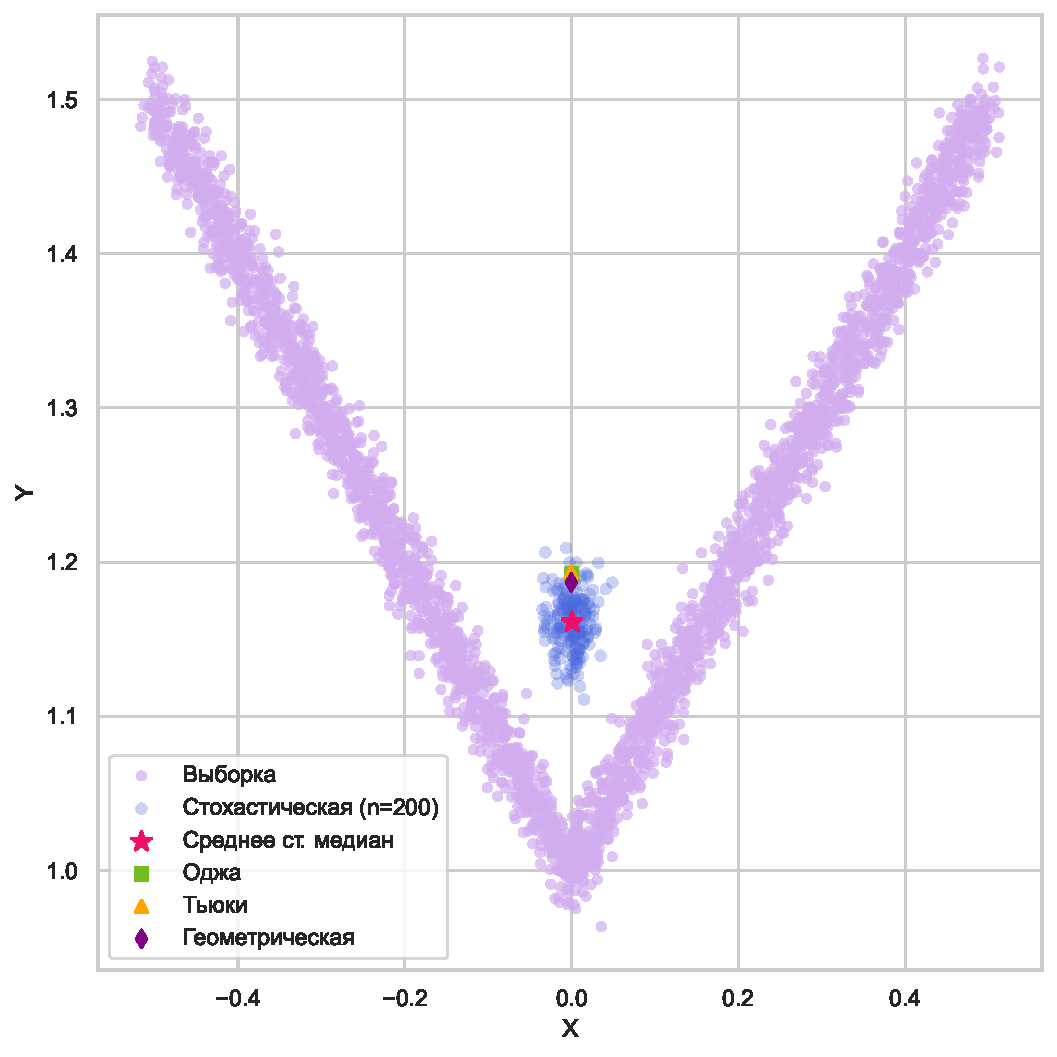
\includegraphics[width=\textwidth]{sample_V_ada.pdf}
    \captionsetup{labelformat=empty}
     \caption{(в) AdaGrad}
     \label{fig:V_rel_ada}
  \end{subfigure}

  \vspace{1ex}

  \begin{subfigure}[b]{0.32\textwidth}
    \centering
    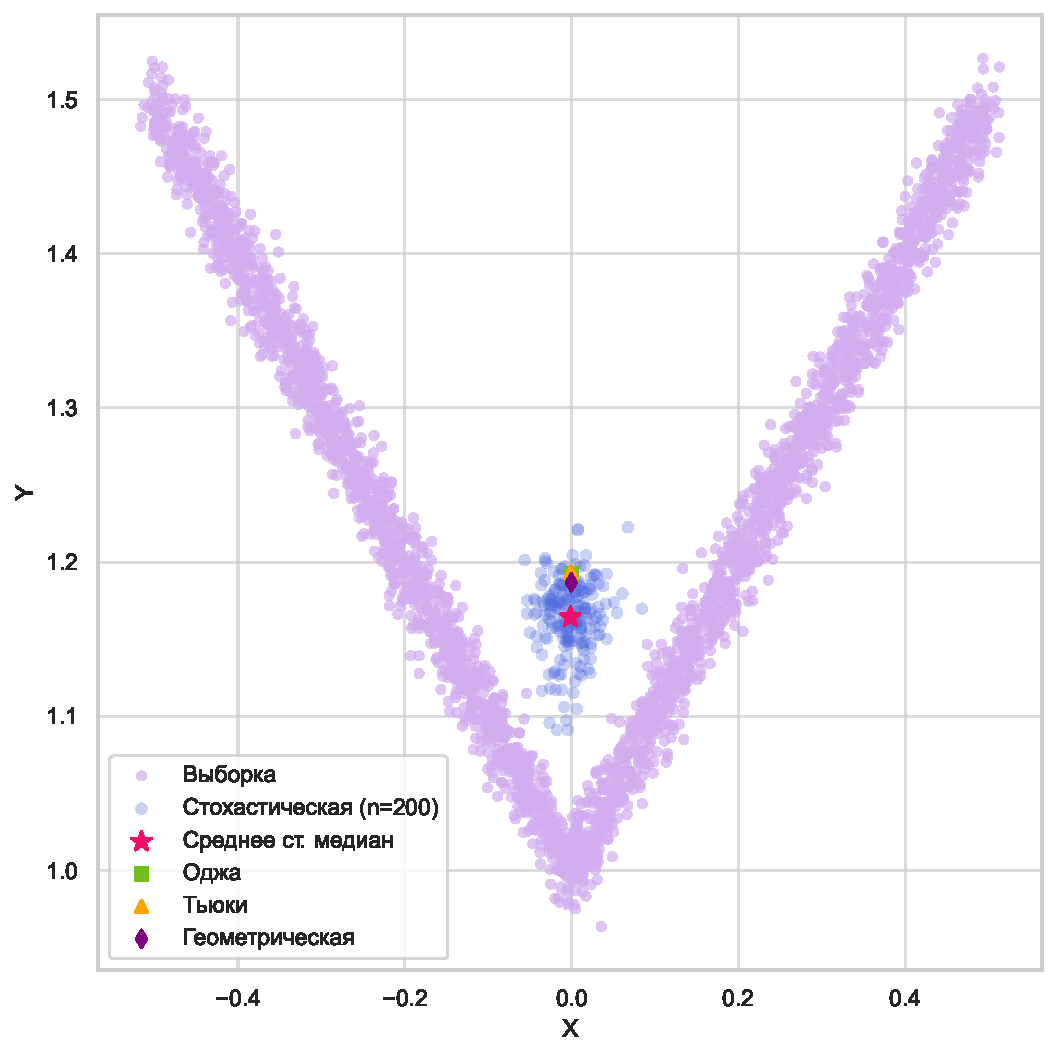
\includegraphics[width=\textwidth]{sample_V_base_avg.pdf}
    \captionsetup{labelformat=empty}
     \caption{(г) Base + Avg}
     \label{fig:V_rel_base_avg}
  \end{subfigure}
  \hfill
  \begin{subfigure}[b]{0.32\textwidth}
    \centering
    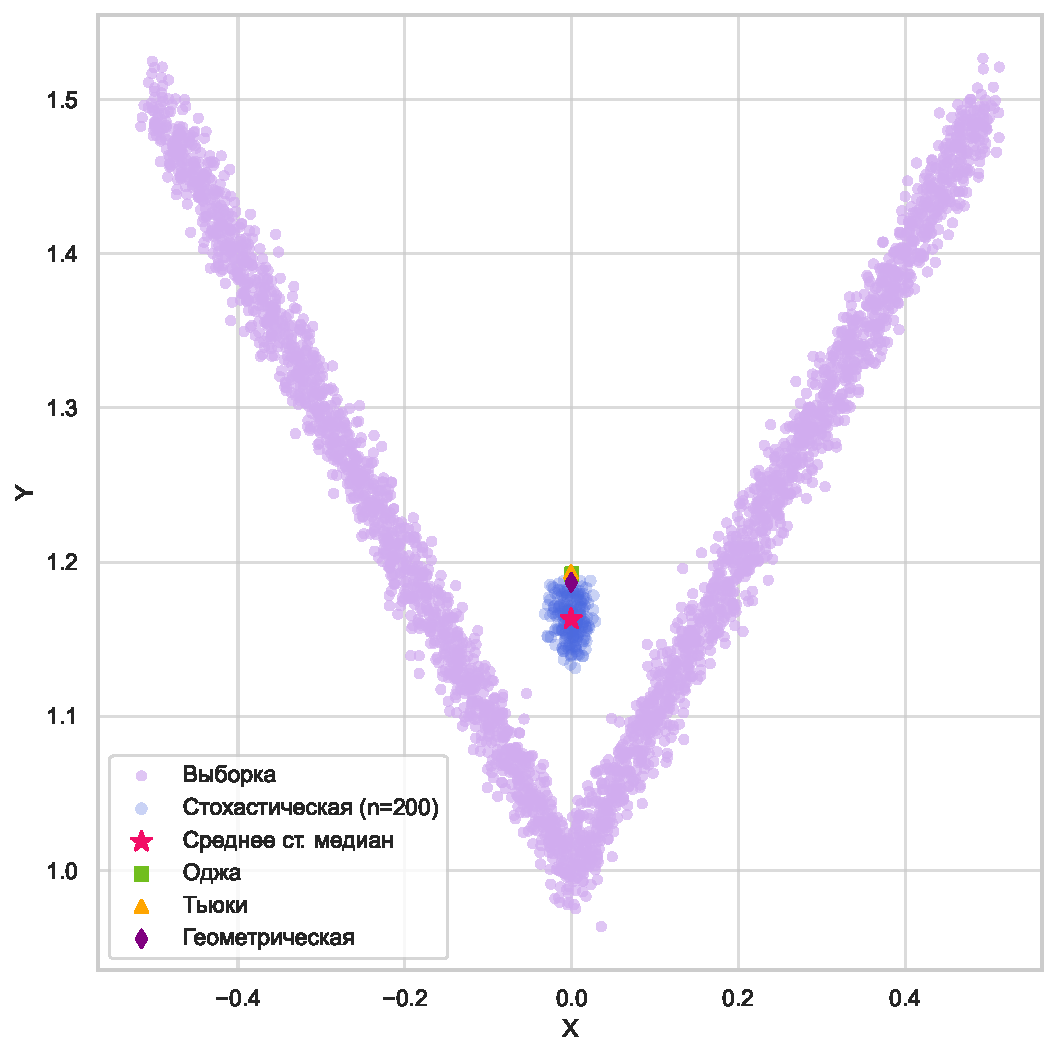
\includegraphics[width=\textwidth]{sample_V_exp_avg.pdf}
    \captionsetup{labelformat=empty}
    \caption{(д) Exp + Avg}
    \label{fig:V_rel_exp_avg}
  \end{subfigure}
  \hfill
  \begin{subfigure}[b]{0.32\textwidth}
    \centering
    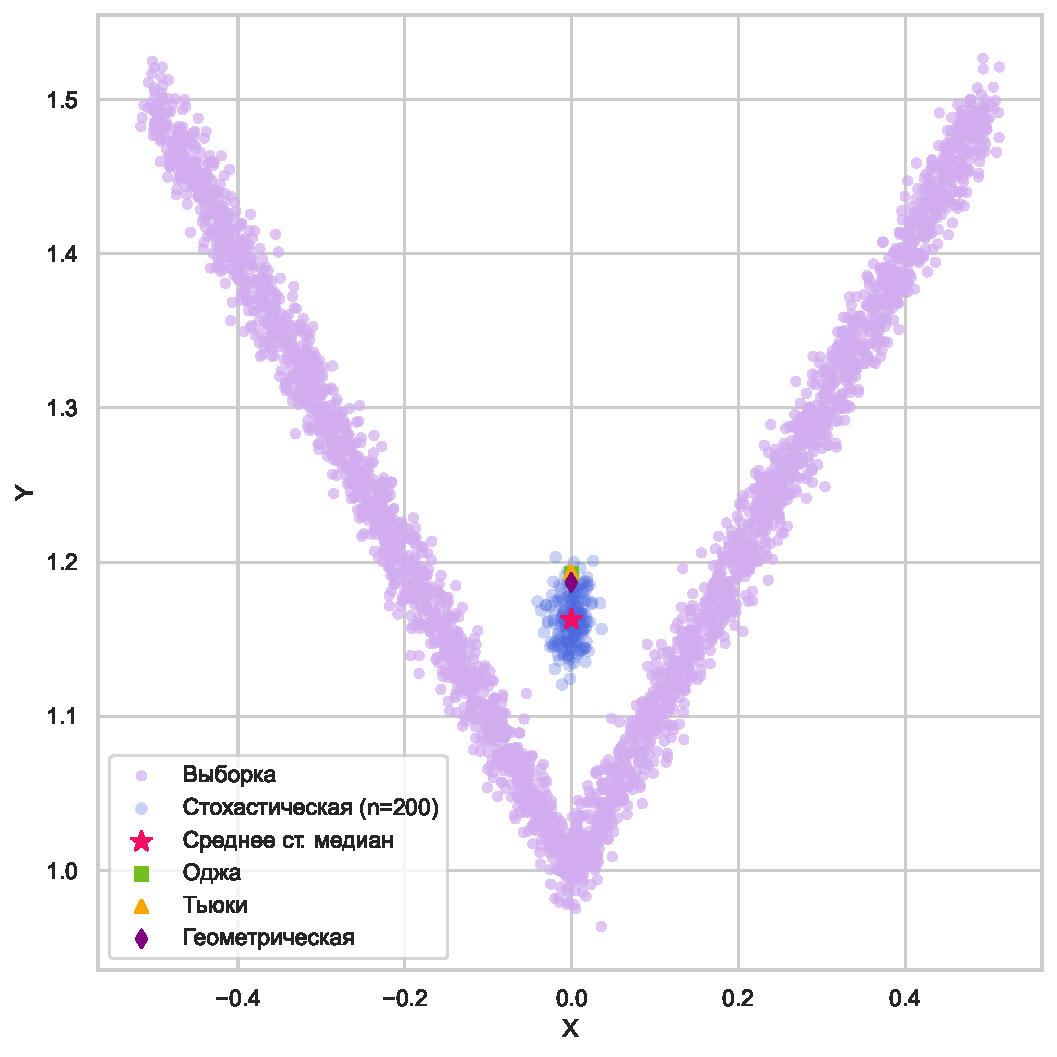
\includegraphics[width=\textwidth]{sample_V_ada_avg.pdf}
    \captionsetup{labelformat=empty}
     \caption{(е) AdaGrad + Avg}
     \label{fig:V_rel_ada_avg}
  \end{subfigure}

  \caption{Результаты работы различных модификаций алгоритма на выборке, образующей букву V.}
 \label{fig:V_comp}
\end{figure}

Из Рисунка~\ref{fig:V_comp} видно, что базовая версия алгоритма (Рис.~\ref{fig:V_rel}) демонстрирует значительный разброс оценок. Полученные значения образуют большое облако точек, вытянутое вдоль вертикального направления. При этом медианы Тьюки, Оджа и геометрическая медиана располагаются достаточно близко друг к другу.

Использование усреднения последних итераций (Рис.~\ref{fig:V_rel_base_avg}) позволяет уменьшить разброс оценок, однако облако точек остается достаточно широким.

Применение экспоненциального сглаживания (Рис.~\ref{fig:V_rel_exp}) приводит к существенному уменьшению разброса. Оценки становятся значительно более сконцентрированными около центра облака.

Наиболее устойчивые результаты наблюдаются при совместном использовании сглаживания и усреднения (Рис.~\ref{fig:V_rel_exp_avg}). В этом случае разброс оценок минимален, а облако точек становится существенно более компактным по сравнению с базовой версией алгоритма.

Модификация AdaGrad (Рис.~\ref{fig:V_rel_ada}) также уменьшает разброс оценок, однако итоговые результаты оказываются менее устойчивыми, чем при использовании экспоненциального сглаживания. Добавление усреднения (Рис.~\ref{fig:V_rel_ada_avg}) дополнительно улучшает ситуацию, однако распределение оценок все равно остается менее компактным по сравнению с методом Exp + Avg.

Таким образом, для выборки данного типа наилучшие результаты демонстрирует модификация с экспоненциальным сглаживанием и усреднением последних итераций.

\subsection{Выборка, образующая букву C}

Рассмотрим также поведение алгоритма на выборке, образующей букву C. В данном случае сравниваются базовая версия алгоритма и модификация с экспоненциальным сглаживанием и усреднением, показавшая наилучшие результаты.

\begin{figure}[!htbp]
  \centering
  \begin{subfigure}[b]{0.45\textwidth}
    \centering
    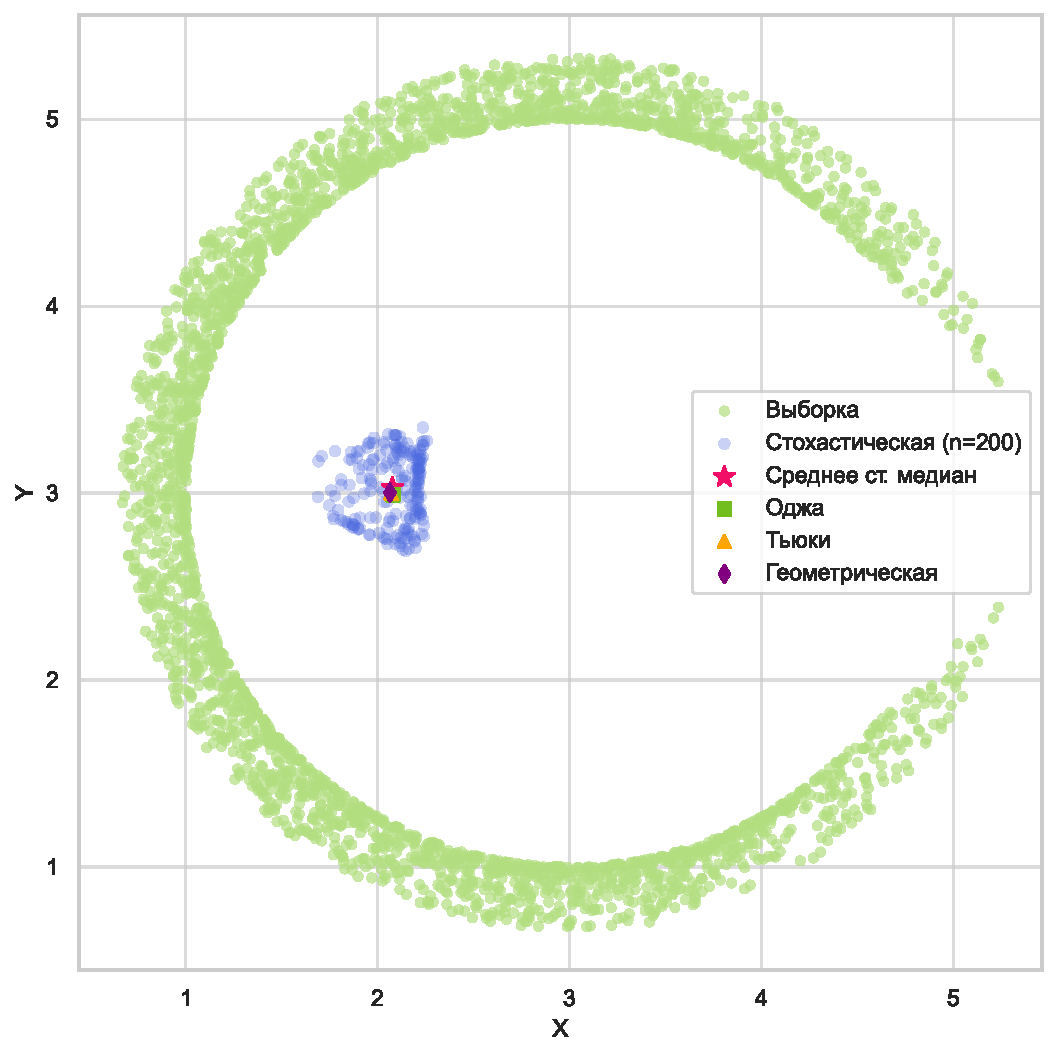
\includegraphics[width=\textwidth]{sample_C_base_new.pdf}
    \captionsetup{labelformat=empty}
     \caption{(а) Base}
     \label{fig:C_rel}
  \end{subfigure}
   \hfill
  \begin{subfigure}[b]{0.45\textwidth}
    \centering
    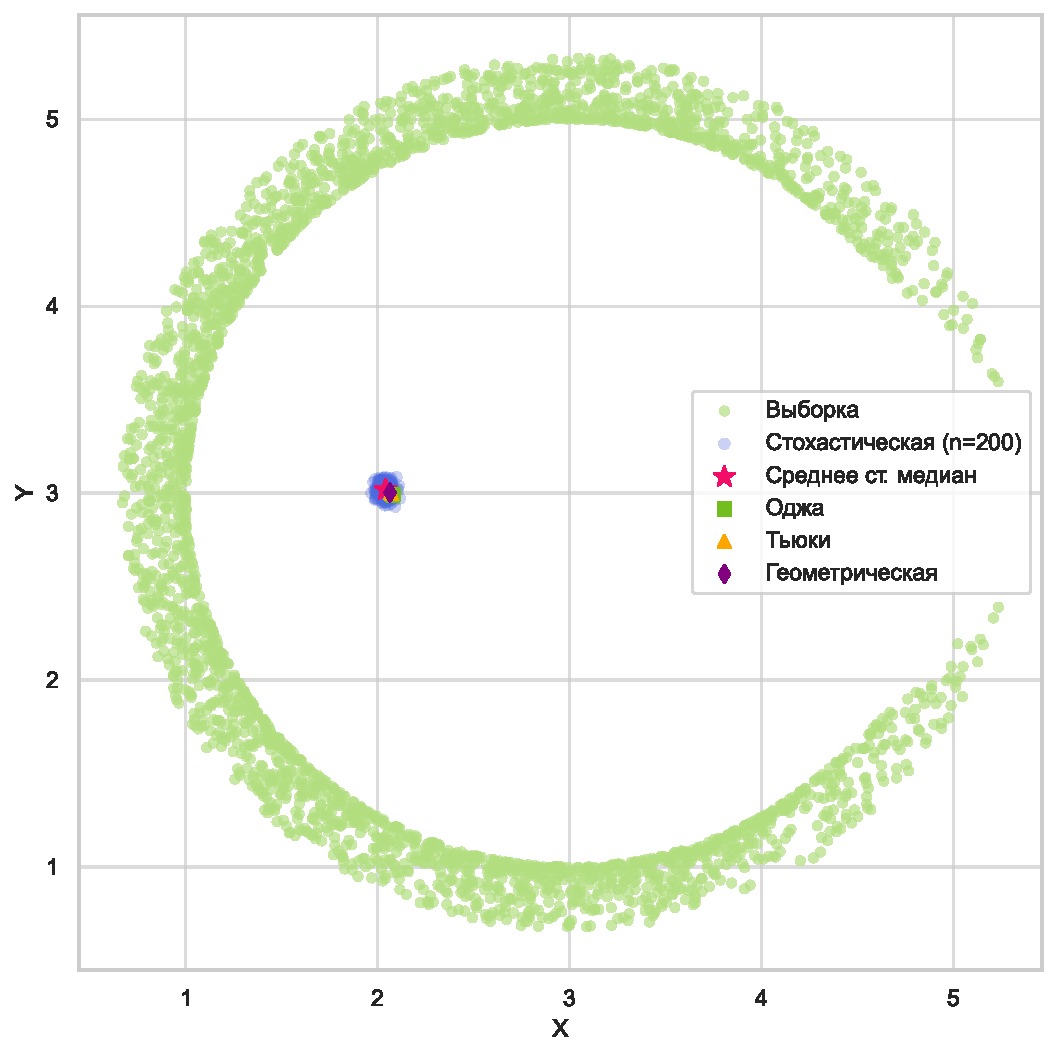
\includegraphics[width=\textwidth]{sample_C_exp_avg.pdf}
    \captionsetup{labelformat=empty}
    \caption{(б) Exp + Avg}
    \label{fig:C_exp_avg}
  \end{subfigure}

  \caption{Результаты работы различных модификаций алгоритма на выборке, образующей букву C.}
 \label{fig:C_comp}
\end{figure}

На Рисунке~\ref{fig:C_comp} видно, что базовая версия алгоритма (Рис.~\ref{fig:C_rel}) не обеспечивает устойчивой сходимости: полученные оценки образуют облако с заметным разбросом.

Использование экспоненциального сглаживания совместно с усреднением (Рис.~\ref{fig:C_exp_avg}) существенно уменьшает размеры облака и делает оценки значительно более стабильными. При этом результаты оказываются близкими к медианам Тьюки, Оджа и геометрической медиане.

Таким образом, даже в случае сложной невыпуклой геометрии модификация Exp + Avg позволяет существенно повысить устойчивость алгоритма.

\subsection{Выборка из вершин вложенных треугольников}

Рассмотрим двумерную выборку из $9$ точек, задающих вершины вложенных равносторонних треугольников:
\begin{align*}
(3; 2)^{\mathrm{T}}, \ (4; 3)^{\mathrm{T}},\ (5; 4)^{\mathrm{T}},\ (11; 2)^{\mathrm{T}},\ (10; 3)^{\mathrm{T}},\ (9; 4)^{\mathrm{T}}, \\ (7; 2+ 4 \cdot \sqrt{3})^{\mathrm{T}},\ (7; 3+ 3 \cdot \sqrt{3})^{\mathrm{T}}, \ (7; 4+ 2 \cdot \sqrt{3})^{\mathrm{T}}.    
\end{align*}

Центр тяжести в данном случае находится в точке $\left(7 ;   \frac{4\cdot\sqrt{3}}{6} + 4\right)^{\mathrm{T}}.$

\vspace{1ex}

На данной выборке базовая версия алгоритма не сходится, это можно увидеть по траектории последовательных приближений на Рисунке~\ref{fig:point_9_traj}.

\begin{figure}[!htbp]
   \centering
    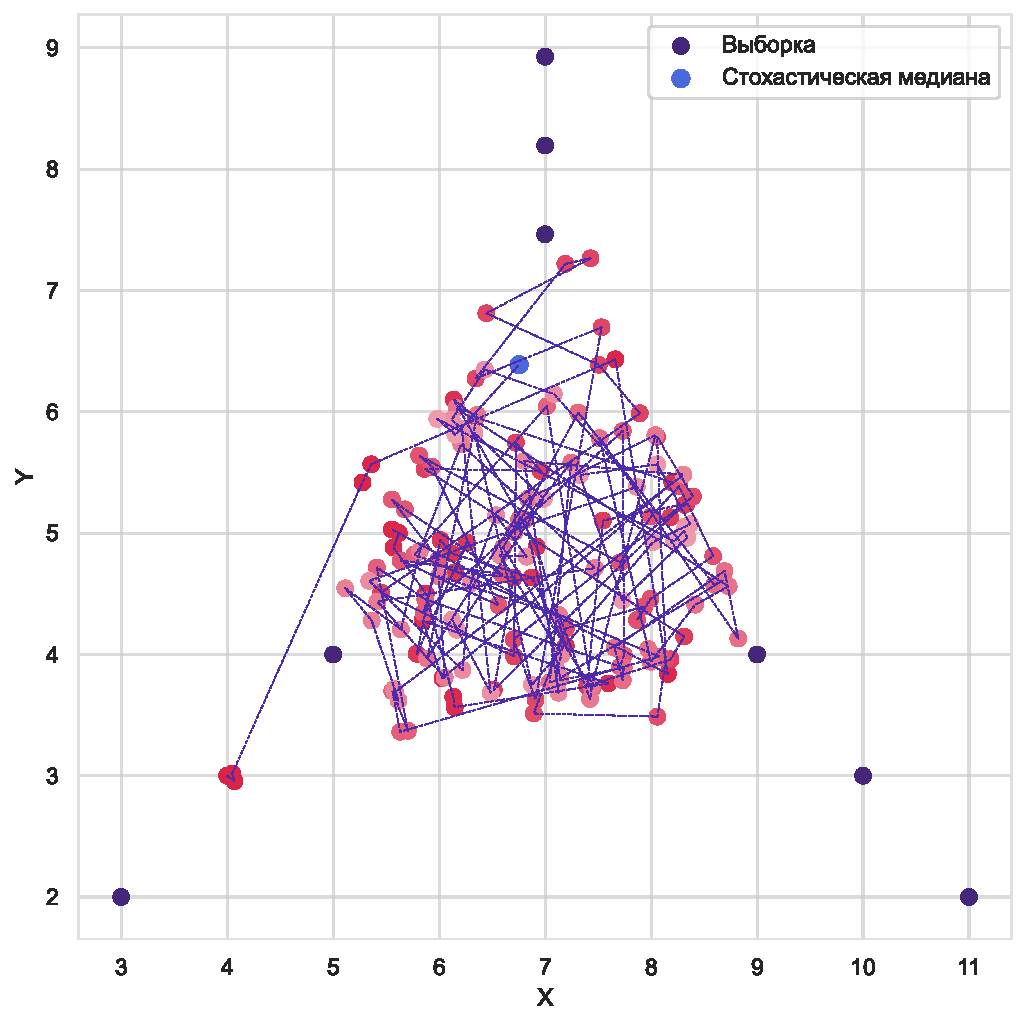
\includegraphics[width=0.5\textwidth]{sample_9point_4.pdf}
    \vspace{-2.75ex}
    
  \caption{Траектория базового алгоритма для выборки из 9 точек.}
  \label{fig:point_9_traj}
\end{figure}

На Рисунке~\ref{fig:point_9_traj} видно, что алгоритм хаотично перемещается между вершинами внутреннего треугольника и не стабилизируется около одной точки. В результате последовательность приближений не демонстрирует сходимости.

Далее сравним базовую версию алгоритма и модификацию AdaGrad с усреднением, которая показала наилучшие результаты для данной выборки.

\begin{figure}[!htbp]
  \centering
  \begin{subfigure}[b]{0.45\textwidth}
    \centering
    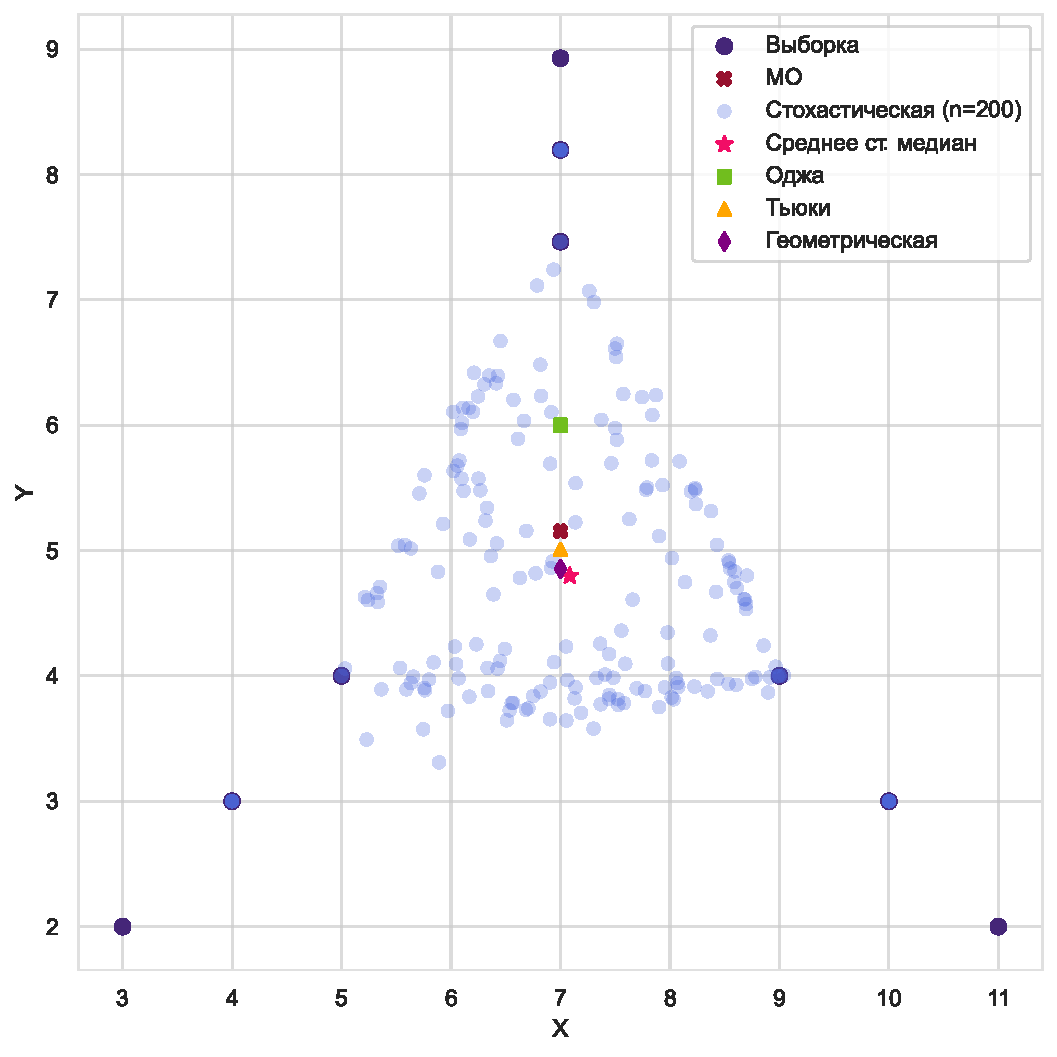
\includegraphics[width=\textwidth]{sample_9point_rel_crit_new.pdf}
    \captionsetup{labelformat=empty}
     \caption{(а) Base}
     \label{fig:9point_rel}
  \end{subfigure}
   \hfill
  \begin{subfigure}[b]{0.45\textwidth}
    \centering
    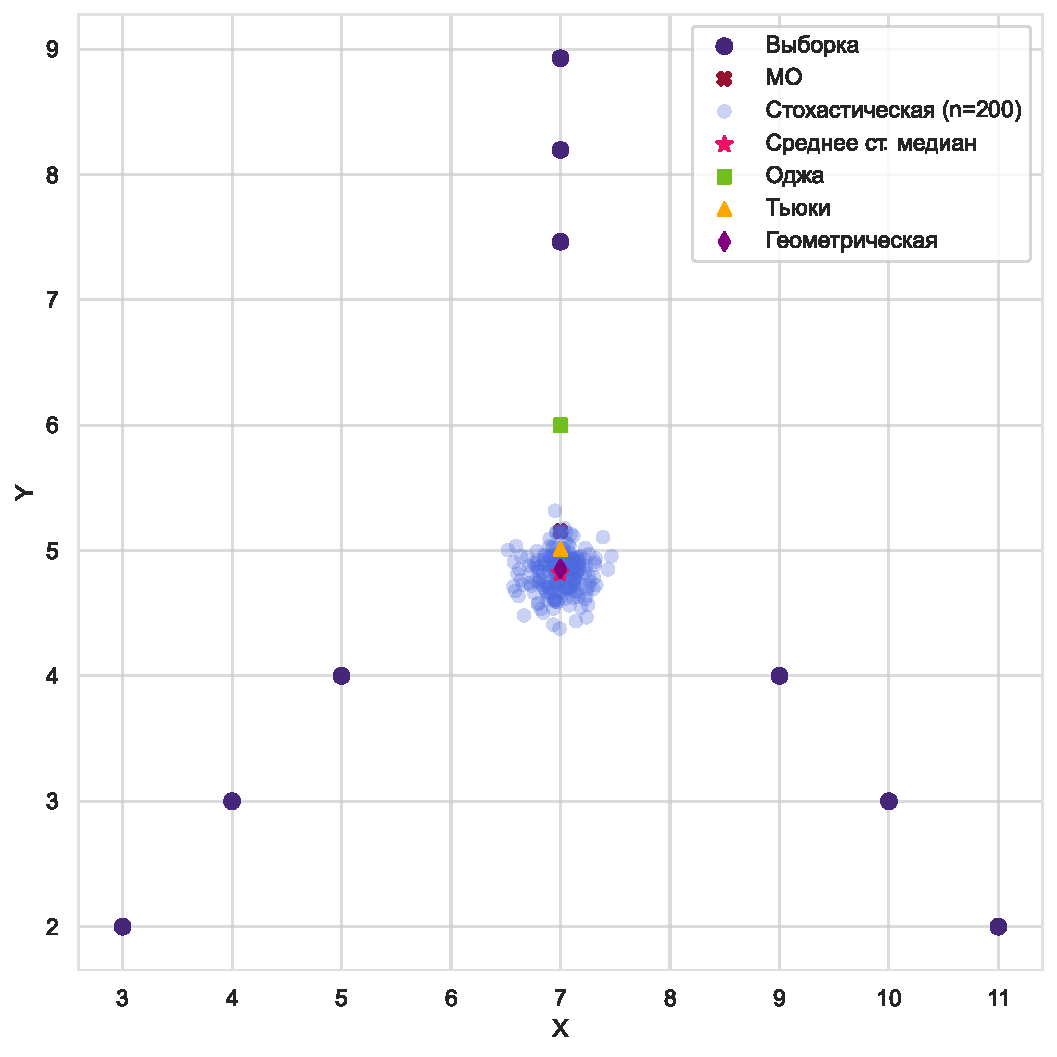
\includegraphics[width=\textwidth]{sample_9point_rel_crit_ada.pdf}
    \captionsetup{labelformat=empty}
    \caption{(б) AdaGrad + Avg}
    \label{fig:9point_exp_ada}
  \end{subfigure}

  \caption{Результаты работы модификаций алгоритма на выборке из вершин вложенных равносторонних треугольников.}
 \label{fig:9point_comp}
\end{figure}

На Рисунке~\ref{fig:9point_comp} видно, что базовая версия алгоритма (Рис.~\ref{fig:9point_rel}) дает большой разброс оценок внутри внутреннего треугольника.

Использование AdaGrad совместно с усреднением (Рис.~\ref{fig:9point_exp_ada}) позволяет существенно уменьшить разброс оценок и получить компактное облако точек около центра распределения.

Таким образом, рассмотренные примеры показывают, что базовая версия стохастического алгоритма может испытывать трудности со сходимостью на выборках со сложной формой. Однако использование модификаций траектории, особенно экспоненциального сглаживания и адаптивного выбора шага совместно с усреднением, позволяет значительно повысить устойчивость алгоритма и уменьшить разброс оценок.